\documentclass[a4paper, 11pt]{article}
\usepackage{fullpage, soul, listings, amssymb, hyperref, graphicx, qtree}
\title{ Semantic Parser \\
        \normalsize \ \\
		\normalsize 6.S083 Fall 2015 Final Project \\ [25pt]
}
\author{Jessica Kenney\\\today}
\date{}
\lstset{basicstyle=\footnotesize\ttfamily,breaklines=true}
\begin{document}
\maketitle
\tableofcontents
\newpage\section{Overview}
Semantic Parser translates sentences of English into sentences of predicate logic, and then generates conclusions or checks given conclusions. For example, generating conclusions:

\noindent Input:\\
\indent ``John is both a man and a farmer.\\
\indent Every man eats."\\

\noindent Translation:\\
\indent (Mj $\wedge$ Fj)\\
\indent ($\forall$x)(Mx $\rightarrow$ Ex)\\

\noindent Generated Conclusions:\\
\indent Ej\ \ ``John eats"\\
\indent ($\exists$x)(Fx $\wedge$ Ex)\ \ ``There is some entity x such that x is a farmer and x eats"\\

\noindent And validating conclusions:\\
\noindent Input:\\
\indent ``Every man eats.\\
\indent Marc is a man.\\
\indent Therefore, Marc drinks a coke."\\

\noindent Translation:\\
\indent ($\forall$x)(Mx $\rightarrow$ Ex)\\
\indent Mm\\
\indent $\therefore$ ($\exists$x)(Cx $\wedge$ Dmx)\\

\noindent Validity Testing:\\
\indent INVALID\\
\indent Counterexample: Universe(\\
\indent\indent Domain: m, hypothetical\_a \\
\indent\indent Set C: \{hypothetical\_a\}\\
\indent\indent Set M: \{m\}\\
\indent\indent Set E: \{m\}\\
\indent\indent Set D: \{\}\\
\indent  )\\

In the above counterexample universe, Marc is a man and Marc eats, and there is a coke, but Marc doesn't drink it. This universe is possible given the two priors, and the conclusion is false in this universe, so the conclusion is invalid.

\subsection{Running}
The system is written in Scala and takes a file name as input.
To run, you need to first install \href{http://www.scala-sbt.org/}{sbt}.
The project code is on github at \url{https://github.com/seveneightn9ne/semantic-parser}.
To download and run the code:
\begin{lstlisting}
  $ git clone https://github.com/seveneightn9ne/semantic-parser.git
  $ cd semantic-parser
  $ sbt "run input/multiple.txt"
\end{lstlisting}
This will run with the input coming from the file \texttt{input/multiple.txt}. There are many other example inputs there that you can try, too.

An input file should contain a sequence of sentences in the present tense.
If a sentence starts with ``Therefore,'' it will be validated as an attempted conclusion.
If there are no sentences that start with ``Therefore,'' it will try to generate some conclusions for you.
There is no support (yet) for prepositional phrases or adjectives.

\subsection{System Diagram}
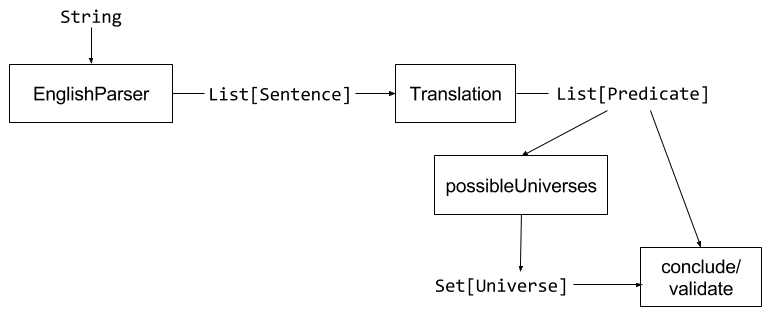
\includegraphics[width=\textwidth]{diagram.png}\\
This diagram shows what happens in the easy case.
The \texttt{EnglishParser} returns only one unambiguous list of \texttt{Sentence}s, and they are all able to be translated into \texttt{Predicate}s. The \texttt{Predicate}s are used to generate possible universes, which are then used to evaluate the conclusions (either made up conclusions, or ones provided in the input).

Often, there will be multiple possible parses for the \texttt{Sentence}s.
In this case, we check if all interpretations are translatable (and that they translate to different \texttt{Predicate}s).
If they do, we have an unrecoverable ambiguity, and it will print the ambiguous \texttt{Sentence} trees and \texttt{Predicate}s to the console, and give up on conclusions.

Sometimes, there are too many entities and relations (sets) introduced by the predicates, so that the number of possible universes becomes very large. The system only does conclusion/validation by searching for counterexamples, so it generates all possible universes, and filters for ones in which the predicates are true. When the number of universes is more than $2^{22}$, the system does not attempt to generate them, and fails with a message to the console.

\subsection{Code Layout}
All the Scala code is under \texttt{src/main/scala/}.
The \texttt{XP} and \texttt{Xbar} datatypes representing English sentences are all in the \texttt{EnglishStructure/} folder.
The \texttt{Predicate} datatype representing logical predicates is in \texttt{PredicateCalculus/Predicates.scala}.


\section[X-bar Sentence Representation]{X-bar Sentence Representation\\
	\normalsize \texttt{src/main/scala/EnglishStructure/*}}
The system uses a simplified version of X-bar syntax. A \texttt{Sentence} is actually just a \texttt{VP}, so there is no \texttt{TP} or \texttt{CP}. There is also no notion of movement. This restricts the parseable sentences by a lot, but allows for a simpler and more readable grammar. It would not actually be difficult to expand the system to use tense, but it might not be very useful.

Another design decision was to make the noun the head of a determiner-noun phrase, instead of the determiner, because this seemed the most straightforward to me when I started. However, when it came to translation, it turns out that the logical translation of a determiner-noun phrase is basically entirely determined by the determiner (consider ``every boy ...'' which translates to ``($\forall$x)(Bx $\rightarrow$ ...)'', versus ``some boy ...'' ``($\exists$x)(Bx $\wedge$ ...)''. So it probably would have been better to switch to determiner-headed phrases here.

\subsection[XP]{XP\\
	\normalsize \texttt{src/main/scala/EnglishStructure/XP.scala}}
There is a type \texttt{XP}, which is parameterized on the types of the Specifier, Head, Complement, and Adjunct. So for example a \texttt{VP} is an \texttt{XP[Noun, Verb, Noun, Adverb]}, because its spec and complement are \texttt{NP}s, and its adjunct type is an \texttt{AdvP}. The implemented \texttt{XP} subtypes are:
\begin{itemize}
\item \texttt{VP} extends \texttt{XP[Noun, Verb, Noun, Adverb]}
\item \texttt{NP} extends \texttt{XP[Determiner, Noun, Verb, Preposition]}
\item \texttt{DP} extends \texttt{XP[Noun, Determiner, Word, Word]}
\item \texttt{PP} extends \texttt{XP[Word, Preposition, Noun, Word]}
\item \texttt{AdvP} extends \texttt{XP[Word, Adverb, Word, Adverb]}
\end{itemize}

In the parameterizations, the use of \texttt{Word} means that the phrase cannot have that thing. For example, PPs do not have specifiers or adjuncts. Each \texttt{XP} contains an optional specifier \texttt{XP}, and a head, which is either an \texttt{Xbar} or a conjunction of two \texttt{XP}s.

Although the definition for \texttt{PP}s was written, the system does not use them (the parser does not know how to parse prepositional phrases).

\subsection[X-bar]{Xbar\\
	\normalsize \texttt{src/main/scala/EnglishStructure/XP.scala}}
The \texttt{Xbar} types are analogous to the \texttt{XP} types. They contain a head which is either an \texttt{Xbar} or a \texttt{Word}. They have an optional complement \texttt{XP} and an optional adjunct \texttt{XP}. While a single \texttt{Xbar} cannot have both a complement and an adjunct, this is enforced at runtime as opposed to being enforced by the type system.

\subsection[Words]{Words\\
	\normalsize \texttt{src/main/scala/EnglishStructure/*}}
There are two types of words: open class, and closed class words. Closed class words, like determiners, are implemented as an \texttt{Enumeration} of possible values. Open class words such as nouns can take any \texttt{String} as their value, and they have some simple morphology attached, such as a plural marker. Verbs have a marker for plural agreement with the subject.

The advantage of the open class/ closed class approach is that the system can use any names or made up words in sentences that are still understandable as English. A disadvantage is that it cannot handle any special case rules, such as ``men'' being the plural for ``man''. If you want it to recognize that those words represent the same set of entities, then you have to write ``men'' as ``mans'' instead. While it would be possible to include special cases such as these in the grammar, I decided for the simplicity and readability of the grammar to not handle these cases. 

As mentioned above, there is no tense on verbs, they are always interpreted as present tense.

\subsection[Conjunctions]{Conjunctions\\
	\normalsize \texttt{src/main/scala/EnglishStructure/XP.scala}}
Conjunctions seem to be the unfortunate outliers of X-bar theory. I implemented them as a \texttt{ConjP} phrase parameterized on the type of \texttt{XP} phrase it contains (and is contained by). \texttt{ConjP}s have an optional \texttt{Preconj} (such as ``either,'' ``both''), two \texttt{XP} subphrases, and a conjunction word (``and'' or ``or''). So an \texttt{XP} is headed by either an \texttt{Xbar} or a \texttt{ConjP[XP]}. There is a runtime restriction that an \texttt{XP} headed by a \texttt{ConjP} cannot have a spec, but this isn't restricted by the type system.

Also, every \texttt{XP} type has to allow conjunctions (this is possible to get around, but would make messier code), so you could construct a \texttt{Sentence} such as ``Either the or a boy eats cake'' (Where the determiner is a conjunction).


\section[Predicate Calculus Representation]{Predicate Calculus Representation\\
	\normalsize \texttt{src/main/scala/PredicateCalculus/Predicates.scala}}

\subsection{Entities}
There are two subtypes of \texttt{Entity}: \texttt{EntityConstant} and \texttt{EntityVariable}. \texttt{EntityConstant} can represent either an individual constant, such as ``j'' representing the entity John, or a hypothetical such as ``hypothetical\_a'' which are generated when creating universes under which to evaluate predicates, so that a premise set with no constants can still be evaluated. \texttt{EntityVariable}s represent the variables bound by \texttt{Existential}s and \texttt{Universal}s.

\subsection{Relations}
Within \texttt{Relation}s, there are unary and binary relations. Within unary relations, there are what I called is-a-relations, that represent nouns, and does-relations, which represent verbs. The \texttt{Relation}s themselves do not hold any entities in them; \texttt{Universe}s assert relationships between \texttt{Relation}s and \texttt{Entity}s.

There is no identity relation, so for example you couldn't represent the sentence ``Marc is the only man who eats cake.'' That would be an infinite relation, which has a true/false assertion for every possible pair of entities. All the relations in this system are finite, so this limits the system from being ``full'' predicate calculus and therefore avoids the problems associated with \href{https://en.wikipedia.org/wiki/G\%C3\%B6del's\_incompleteness\_theorems\#First\_incompleteness\_theorem}{Godel's Incompleteness Theorem} and allows me to be able to deterministically validate proofs.
\subsection{Predicates}
\texttt{Predicate} is a recursive datatype with the following subtypes:
\begin{itemize}
	\item \texttt{Atom}, which takes an \texttt{Entity} and \texttt{UnaryRelation}, as in the predicate ``Wa'' which is the translation of the sentence ``Adam walks.''
	\item \texttt{BinaryAtom}, which takes an \texttt{Entity} and \texttt{BinaryRelation}, as in the predicate ``Lab'' which is the translation of the sentence ``Adam loves Bob.''
	\item \texttt{Negation}, which takes a \texttt{Predicate}, as in ``$\neg$Wa'' which is the translation of the sentence ``Adam doesn't walk.''
	\item \texttt{Conjunction}, which takes two \texttt{Predicate}s, as in ``(Mj $\wedge$ Fj)'' which is the translation of the sentence ``John is both a man and a farmer.''
	\item \texttt{Disjunction}, which takes two \texttt{Predicate}s, as in ``(Mj $\vee$ Fj)'' which is the translation of the sentence ``John is either a man or a farmer.''
	\item \texttt{Existential}, which takes an \texttt{EntityVariable} and a \texttt{Predicate}. It asserts that there is some entity which satisfies the predicate, as in ``($\exists$x)Mx'' which is the translation of the sentence ``There is a man.''
	\item \texttt{Universal}, which takes an \texttt{EntityVariable} and a \texttt{Predicate}. It asserts that all entities satisfy the predicate, as in ``($\forall$x)(Mx $\vee$ Wx)'' which is the translation of the sentence ``Everyone is a man or a woman.''
	\item \texttt{Conditional}, which takes a \texttt{Predicate} antecedent and a \texttt{Predicate} consequent, as in ``($\forall$x)(Bx $\rightarrow$ $\neg$Gx)'' which is the translation of the sentence ``No boys are girls.''
	\item \texttt{Biconditional}, which takes two \texttt{Predicate}s, as in ``($\forall$x)(Vx $\leftrightarrow$ Fx)'' which would be the translation of the sentence ``All vegetarians are feminists, and vice versa,'' though there are no translation rules that create biconditionals.
    \item \texttt{Conclusion}, which takes a \texttt{Predicate} $\phi$ and represents ``$\therefore \phi$''. Its only purpose is to represent that the predicate is an attempted conclusion, and it is the translation of sentences that start with ``therefore.''
\end{itemize}

\texttt{Predicate}s can be evalutated given a \texttt{Universe}, returning \texttt{true} or \texttt{false}. They can also be translated back to English, but this is done in a simple recursive manner directly to text, instead of using translation rules.

\subsection[Naming]{Naming\\
	\normalsize \texttt{src/main/scala/PredicateCalculus/UniqueDesignations.scala}}
When a new relation or entity is introduced, it needs an appropriate name generated. \texttt{UniqueDesignations} provides a global namespace, so you can request a name to be made from a string and it will make the best name that hasn't been used yet. For the variable names in existentials and universals, you pass in a \texttt{Context} which will include any variables that are already bound. That way, different sentences can reuse the same variable (there's no global context for variables).

\section[Universes]{Universes\\
	\normalsize \texttt{src/main/scala/PredicateCalculus/Universe.scala}}
    A \texttt{Universe} (also known as an interpretation) represents a complete description of the truth value of atomic predicates with a given set of entities and relations. So, for example if the only relation is R and the only entity is e, then the universe would say that ``Re'' is either true or false.

\section[CFG Parser]{CFG Parser\\
	\normalsize \texttt{src/main/scala/EnglishParser.scala}}
Scala provides a native parser-combinator library, but I instead used an implementation of the GLL\cite{GLL} algorithm. It can handle even left-recursive grammars in worst-case O$(n^3)$ time. More importantly, it parses nondeterministically, and so allows multiple parses as results. This is essential for being able to parse a natural language, and allows the grammar itself to be written in a very natural way, as opposed to having to manually resolve left-recursion in the grammar.

The grammar itself has explicit rules matching the closed class words, such as determiners, existential ``there'', and ``therefore''. The open-class words like nouns are restricted to not be any of the closed class words, which helps in restricting the valid parses by a lot.

\section[Sentence Translation]{Sentence Translation
	\\ \normalsize \texttt{src/main/scala/Translation.scala}}
The \texttt{translate} function pattern matches on various \texttt{XP} and \texttt{Xbar} structures that it recognizes, and turns them into \texttt{Predicate}s recursively. For example, the sentence ``Every boy who eats, eats cake.'':\\
\Tree [.VP [.NP [.DP Every ] [.N' [.N boy ] [.VP [.NP who ] [.V' eats ] ] ] ] [.V' [.V eats ] [.NP cake ] ] ] \\
This sentence would match the rule that recognizes: \\
\Tree [.VP [.NP [.DP Every ] [.N' ... ] ] [.V' ... ] ]\\
So it would translate the sentence as ``($\forall$x)(\texttt{translate(nbar,x)} $\rightarrow$ \texttt{translate(vbar,x)})'', recursively finding the translations for the N' and V', and passing down the variable \texttt{x} as a \texttt{SubjectContext} object.

\section[Generating Conclusions]{Generating Conclusions
	\\ \normalsize \texttt{src/main/scala/Main.scala}
	\\ \normalsize \texttt{src/main/scala/PredicateCalculus/Conclusions.scala}}
To generate conclusions, there are five steps.
\begin{enumerate}
	\item \textbf{Generate all possible universes.} To do this we first get all of the \texttt{EntityConstant}s, \texttt{UnaryRelation}s, and \texttt{BinaryRelation}s in the predicates, plus another two hypothetical \texttt{EntityConstant}s. The two hypotheticals are so that any universal conclusions are actually universal, and not just things that happened to be true for the given entities. For example, if the only given predicate is ``($\exists$x)Wx'', then there would be no entities, so you couldn't find any universe in which the premise is true. But if you added only one hypothetical entity, then you restricted to universes where the prior is true, then you would conclude that ``($\forall$x)Wx'', which is not true. Therefore, we add two hypothetical entities, which avoids this problem.
    
 	Unfortunately, generating all possible universes gets really huge really fast. The number of universes is $2^{eu} * 2^{e^2b} = 2^{e^3ub}$, where $e$ is the number of entities (including the 2 hypotheticals), $u$ is the number of unary relations, and $b$ is the number of binary relations. Whenever this number is larger than $2^{22}$ the program terminates immediately instead of trying to compute, because on my computer the JVM runs out of memory and crashes with $2^{22}$ universes. I tried to improve this by incrementally generating universes, so a partial universe could answer ``I don't know'' to an assertion, but it was very complicated and didn't seem to improve the runtime by enough to be worth it.
    \item \textbf{Filter universes for ones in which all the predicates are true.} This is just straightforward filtering.
    \item \textbf{Generate a lot of conclusions.} 
    I generate all possible atoms and their negations, universal atoms, 
    existential atoms, universal conditionals on atoms (of the form 
    ``($\forall$x)($\phi$x $\rightarrow$ $\rho$x)''), and existential conjunctions
    (``($\exists$x)($\phi$x $\wedge$ $\rho$x)''). 
    Any time I wish the system concluded something, 
    I add the form of that conclusion to this set of generated conclusions.
    \item \textbf{Filter for conclusions which are true under all possible universes.} 
    Once again, straightforward filtering.
    \item \textbf{Filter for conclusions that are ``interesting.''} 
    This means I take out conclusions that are true given only one of the premises,
    conclusions that are logically equivalent to each other, 
    and conclusions that entail each other, keeping the most specific conclusion. 
    For example, I would discard ``($\exists$x)Ex'' (There is someone who eats) 
    in favor of ``Ej'' (John eats).
\end{enumerate}
It would also be possible to generate conclusions by performing the proof procedure rules given in 24.241 (Logic). 
Rules like universal specification, quantifier exchange ($\neg$($\forall$x)$\phi$ = ($\exists$x)$\neg\phi$), and tautological consequence. 
Perhaps this can be considered future work.

\section[Validating Conclusions]{Validating Conclusions
	\\ \normalsize \texttt{src/main/scala/Main.scala}
	\\ \normalsize \texttt{src/main/scala/PredicateCalculus/Conclusions.scala}}
Validating conclusions is very similar procedurally to the steps of generating conclusions.
\begin{enumerate}
\item \textbf{Generate all possible universes.} This is the same as steps 1-2 above.
\item \textbf{Assert that each conclusion is true in all possible universes.} 
If there exists a universe in which all the priors are true but a conclusion is false, 
then that universe will be presented as a counterexample, and the conclusion is invalid. 
Otherwise, the conclusion is valid.
\end{enumerate}
\section{System Evaluation}
The system works well for small inputs in the forms that I have tested. 
The translation from \texttt{Sentence}s to \texttt{Predicate}s is quite specific and not super generalizable, so novel inputs have a good chance of tripping it up. 
Part of this I think is due to using noun headed phrases instead of determiner headed phrases, so you have to look deeper into the structure of a phrase to know what to do with it.

The amount of possible universes is the other main weakness of the system.
I tried a lot of various ways of generating fewer universes, and some helped a lot
(for example, you only need two hypothetical entities total, as opposed to two per
universal or existential predicate). But overall the time it takes is still a hugely limiting factor. 
\begin{thebibliography}{9}
\bibitem{GLL} Elizabeth Scott and Adrian Johnstone. \emph{GLL Parsing.} \url{http://dotat.at/tmp/gll.pdf}, 2010.
\end{thebibliography}

\end{document}
